% 2019-02-20

\documentclass[10pt]{article}
\usepackage[T1]{fontenc}
\usepackage{amssymb}
\usepackage{amsmath}
\usepackage{graphicx}
% \begin{figure}[h]
% \centering
% \includegraphics[width=6.5in]{folder/photo.png}
% \caption{}
% \label{}
% \end{figure}



\usepackage{tikz}
\usetikzlibrary{arrows}
\usepackage{subfigure}
\usepackage{stackrel}
\usepackage{blindtext}

\usepackage{biblatex}
\addbibresource{library.bib}

\oddsidemargin=0.15in
\evensidemargin=0.15in
\topmargin=-.5in
\textheight=9in
\textwidth=6.25in

\usepackage[colorlinks=true,breaklinks,pdfpagemode=none,linkcolor=blue,citecolor=blue]{hyperref}

\usepackage{enumerate}
% \vspace{-6pt}
% \begin{itemize}
%     \setlength{\itemsep}{0pt}%
%     \setlength{\parskip}{0pt}%
%     \item Item 1
%     \item Item 2
%         \begin{itemize}
%             \setlength{\itemsep}{0pt}%
%             \setlength{\parskip}{0pt}%
%             \item Sublist Item 1
%             \item Sublist Item 2
%         \end{itemize}
%         \item Item 3
% \end{itemize}
% \vspace{-6pt}


\usepackage{enumitem}
\setlist{itemsep=0mm}

\usepackage{amsmath,amsfonts,amssymb,bm}



\begin{document}

   \noindent
   \begin{center}

   \hrulefill
   
   \vspace{5pt}
   
   \makebox[\textwidth]{ {\bf Energy Systems Analysis} \hfill  A.D. Smith 2019}
   \vspace{0pt}
   
   {\Large \hfill  Lecture 16. BEM: Parametric Analysis}
   \vspace{5pt}
   
  
   \hrulefill
   \end{center}

{\center{ \small{      ``Computerized    searching    has    the    
potential  to  automate  the  input  and  output,  evaluate  
many   options,   and   perform   enough   simulations   to    account     for     the     complex     interactions     among      combinations of options.''
\\%[3pt]
\rightline{{\rm --- Ellis, Griffith, Long, Torcellini, and Crawley \cite{Ellis2006-wg}}}}}}

%\bigskip

\section{Parametric analysis for modelers}

We will use the term \textbf{parameter} here in one of its broadest senses, that is, ``any of a set of physical properties whose values determine the characteristics or behavior of something. \cite{noauthor_undated-uq}
''
    
The term \textbf{parametric analysis} encompasses methods for varying model parameters (e.g. through building energy simulation) and, hopefully, learning from the changes in model outputs. Samuelson et al. \cite{Samuelson2016-xw} provide a brief description of the advantages of performing parametric analysis with your simulations during a design process:

\begin{quote}
By utilizing
parametric simulation techniques with today's computing power, a modeler can evaluate numerous potential designs to produce guidance that design teams can use as an informed starting point in the design process. \cite{Samuelson2016-xw}
\end{quote}

Parametric analysis is a closely related concept to \textit{sensitivity analysis}, which we will study more formally in the latter half of this course. A parametric analysis varying one particular variable over a range of values would be the simplest form of a sensitivity analysis, but there are much more complex methods, and the phrase sensitivity analysis usually implies a more formal mathematical quantification of how changes to the input(s) affect the output(s).

Within the discipline of statistics, `parameter' and `parameter statistics' have narrowly defined meanings, so be careful using terms in that context.


\section{Parametric analysis and the built environment}

There are often a number of parameters that can be changed in building energy analysis, both those relating to the design and operation of the building and those related to the conditions it experiences. Here are some examples of parameters related to energy performance  \cite{Shiel2018-xh}: 

\begin{itemize}
    \setlength{\itemsep}{0pt}%
    \setlength{\parskip}{0pt}%
    \item Geometry
    \item Materials
    \item Glazing system (fenestration/windows)
    \item HVAC (system or schedule)
    \item Lighting (system or schedule)
    \item Plug loads (system or schedule)
    \item Occupancy (system or schedule)
    \item Adjacent site conditions
    \item Weather conditions
\end{itemize}

Running simulations for a parametric analysis can allow us to investigate the range of effects of a given change on the outputs we are most interested in (e.g. overall energy use, fuel and electricity costs, carbon emissions). Samuelson et al. \cite{Samuelson2016-xw} describe one of the difficulties with taking advantage of parametric analysis tools during a building design process:

\begin{quote}
    Simulations traditionally used in the building industry require detailed inputs and, therefore, are difficult to employ in early design stages when the pace of design iteration is fast and the simulation inputs include many unknown variables. \cite{Samuelson2016-xw}
\end{quote}

In this quote, they are summarizing the work of Ochoa et al. \cite{Ochoa2009-pn}, who describe specific hurdles for using thermal models for building performance early in the design process:

\begin{quote}
``They require exact data in a stage when designers consider conceptual ideas from a range of options rather than precise details and numbers\ldots The number of possible
configurations can be overwhelming and decisions made in early stages have profound effects on energy and comfort performance. 

It would be desirable to include an accurate energy evaluation system for the first design stages that is capable of modelling the complexity of these systems\ldots[But] most tools are dedicated to evaluate and model a certain finished alternative, not to suggest and evaluate different design options and directions.'' \cite{Ochoa2009-pn}
    
\end{quote}

This is particularly difficult early in the design process, when the most opportunities exist for affecting the ultimate performance of the building. However, in all phases of the design process (including retrofit design for existing buildings), we will benefit from:

\begin{itemize}
    \setlength{\itemsep}{0pt}%
    \setlength{\parskip}{0pt}%
    \item Flexibility in the level of detail included in the model
    \item Narrowing down the number of design parameters to those that can have the most impact on performance \cite{Samuelson2016-xw}
        \item Ability to run many simulations when the range of potential parameter values is large
    \item Easy to use interface for the modeling tool \cite{Ochoa2009-pn}
    \item Visualization tools that clearly illustrate the differences resulting from varying parameters or design choices
    \item Rapid elimination of options that are not feasible or ``dead-ends'' \cite{Ochoa2009-pn}
        \item Changing modeling tools to become more detailed as the design evolves \cite{Samuelson2016-xw}
    \item Integrating expert knowledge and engineering judgement based on experience as model results are evaluated
\end{itemize}



\section{Parametric analysis with OpenStudio}

OpenStudio provides support for parametric analysis through a specially designed interface. This program also has support for running multiple models on the cloud (AWS). The basic steps to use the tool are \cite{noauthor_undated-yz}:

\begin{enumerate}
    \setlength{\itemsep}{0pt}%
    \setlength{\parskip}{0pt}%
    \item Open the Parametric Analysis program --- This is a separate application that was installed in your OpenStudio directly with the OpenStudio interface application).
    \item Name your project --- This will be the name of the directory where your parametric analysis is stored.
    \item Provide a default seed model --- This is the OSM model that will provide a baseline for the parametric analysis.
    \item Provide a default weather file --- This is the EPW file that will provide a baseline for the parametric analysis.
    \item Add measures to your project --- These can be OpenStudio, EnergyPlus, or Reporting measures.
    \item Select measures and create design alternatives --- These are the changes that will be made when the simulations are run.
    \item Run simulations --- Select the design alternatives you want to run and click the simulate button, just like in the OpenStudio interface.
    \item View results --- ``You can open htm report files
in your browser. EnergyPlus and
standard and calibration OpenStudio reports can be found by right
clicking on a design alternative, on
the Results tab, and selecting the
results you want to view.'' \cite{noauthor_undated-ks}
\end{enumerate}

\section{Presenting parametric analysis results}

We often have multiple things that could potentially be varied in our analysis, and we want to be able to present the results in a way that captures more than the variation in a single parameter. For example, Szabo et al \cite{L_Szabo2018-nh} analytically calculated the maximum `heat load' (that is the rate of heat removal that would be necessary for air conditioning, or what we would think of as `cooling load') for a simple reference room. One of the conclusions of their paper was that ``The sensitivity of the heat load depends on the orientation and chosen summer day,'' which isn't something we can directly put into practice without more details. Figure \ref{gr} show the results obtained for a \textit{glazing ratio} (think window-to-wall ratio) of 20--80\%. Note that in their presentation of these results they are also capturing important differences that are relevant to the design process, and their parametric results between 20\% and 80\% glazing look slightly different depending on these other factors:

\vspace{-3pt}
\begin{itemize}
    \setlength{\itemsep}{0pt}%
    \setlength{\parskip}{0pt}%
    \item The room's orientation was tested in all four cardinal directions.
    \item They considered cooling the room's surfaces and tested the need for cooling on a wall versus on the ceiling.
    \item Symmetric weather days assume that east and west orientations receive the same amount of solar radiation (which was an assumption made in the standard they were using), while asymmetric weather days represent that in their location it is actually the case that ``solar energy yield for East orientation exceeds the data registered for West orientation.'' \cite{L_Szabo2018-nh}
\end{itemize}
\vspace{-3pt}

They have aligned all the wall cooling results on the left and ceiling cooling results on the right, as well as providing one cardinal direction in each row of Figure \ref{gr}. It would have been almost impossible for us to compare across these factors by looking at this figure if the graphs had not been ordered in a logical manner.


            \begin{figure}[h]
     \centering
            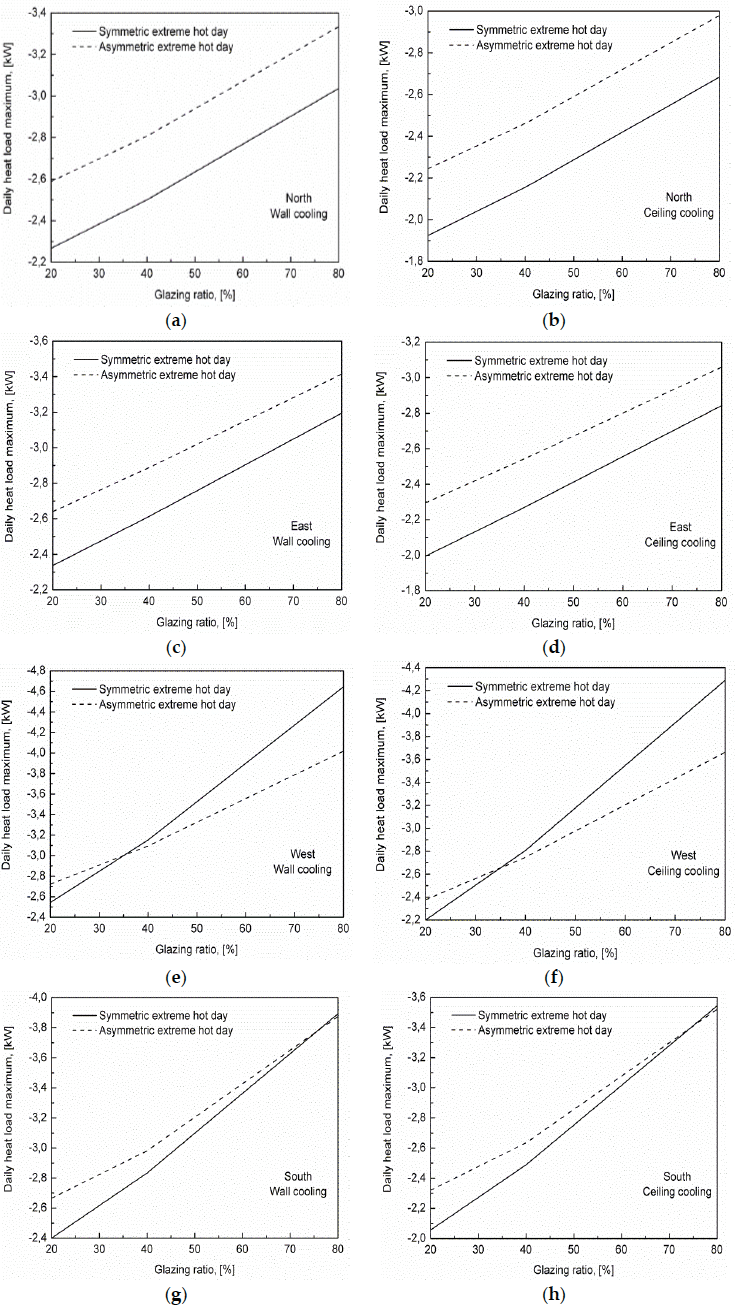
\includegraphics[width=5in]{extras16/glazingratio.png}
            \caption{\footnotesize{Interrelation between glazing ratio and the maximum of the daily heat load. (a) North
orientation and wall cooling; (b) North orientation and ceiling cooling; (c) East orientation and wall
cooling; (d) East orientation and ceiling cooling; (e) West orientation and wall cooling; (f) West
orientation and ceiling cooling; (g) South orientation and wall cooling; (h) South orientation and
ceiling cooling. \cite{L_Szabo2018-nh}}}
            \label{gr}
            \end{figure}


% license
\bigskip

\noindent
\texttt{\footnotesize RESTRICTED PUBLIC LICENSE --- READ BEFORE SHARING. This is a draft version made available by Amanda D. Smith under a Creative Commons Attribution-NonCommercial-ShareAlike license. 
\href{https://creativecommons.org/licenses/by-nc-sa/4.0/}{CC BY-NC-SA 4.0}}

% references

\printbibliography

\end{document}